
\documentclass[tikz, border=1mm]{standalone}

\usepackage{amsmath}

\usepackage{tikz}

\usetikzlibrary{calc,angles,quotes,shapes.geometric}

\begin{document}

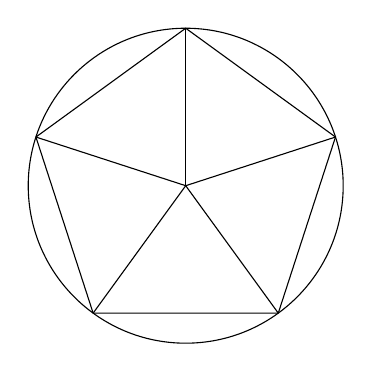
\begin{tikzpicture}[scale=1.0]

	% ---- short method

	%\draw (0,0) circle (2);
	%\node[draw, regular polygon, regular polygon sides=6, minimum size=4cm] at (0,0) {};

	% ---- detailed method

	\def\numsides{5}
	\def\radius{2}
	\def\rotation{90}

	\coordinate (O) at (0,0);
	\draw (O) circle (\radius);

	\foreach \i in {1,...,\numsides} {
		\coordinate (P\i) at ({360/\numsides*(\i-1)+\rotation}:\radius);
	}

	\draw (P1) \foreach \i in {2,...,\numsides} { -- (P\i) } -- cycle;

	\foreach \i in {1,...,\numsides} { \draw (O) -- (P\i); }

	%\foreach \i in {1,...,\numsides} {
		%\node[above right] at (P\i) {$P_{\i}$};
	%}

\end{tikzpicture}

\end{document}
